\documentclass{standalone}

\usepackage{tikz}
\usetikzlibrary{arrows}
\usetikzlibrary{decorations.markings}
\usetikzlibrary{calc}

\begin{document}

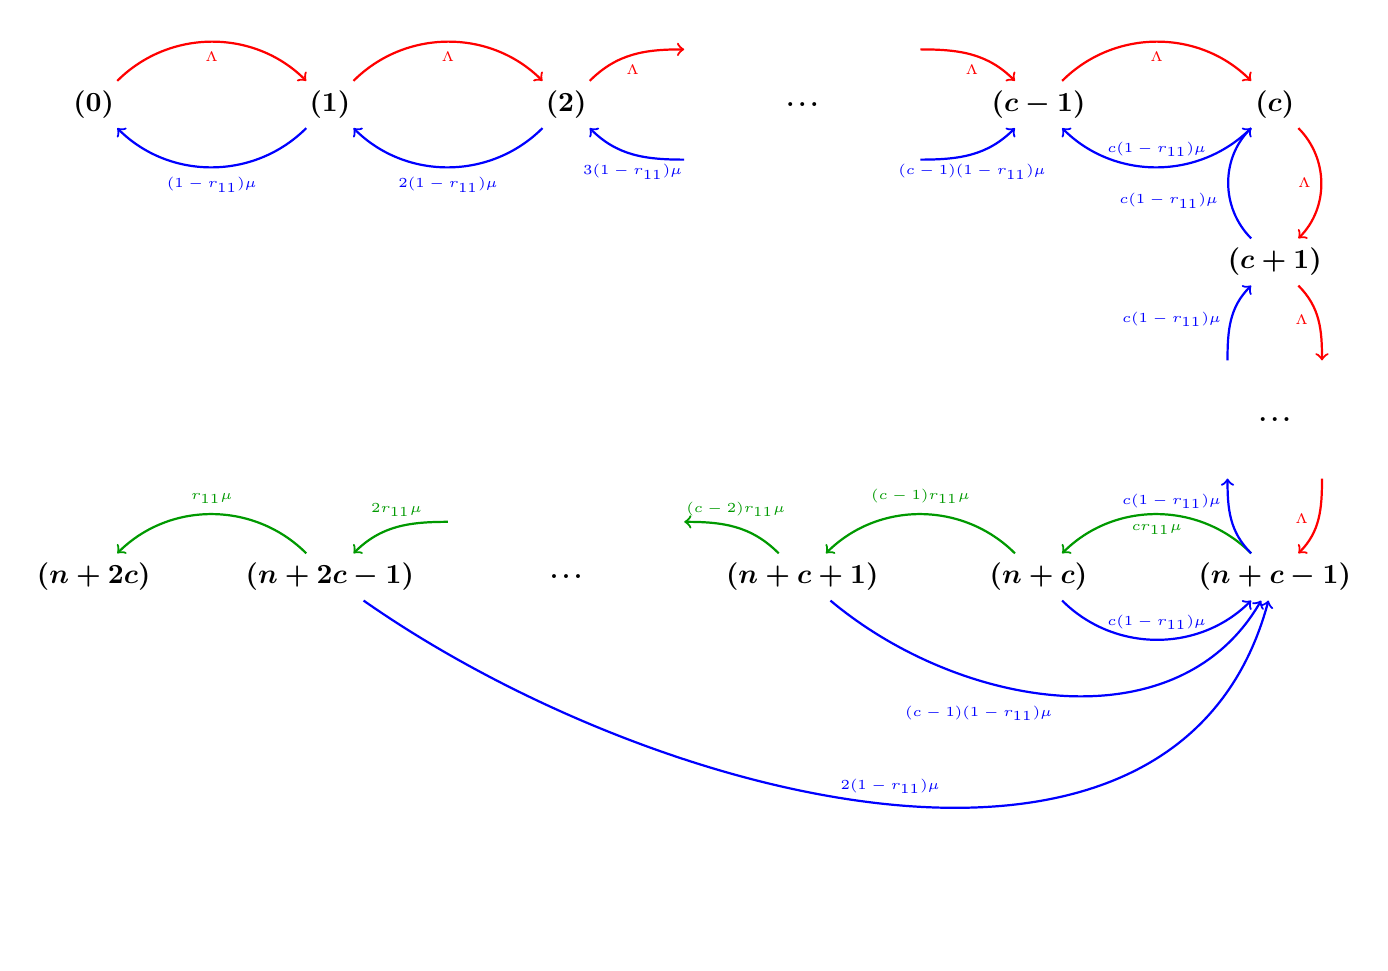
\begin{tikzpicture}
    \tikzstyle{state}=[minimum width=1.5cm, font=\boldmath];
    % First col
    \node (0) at (0,0) [state] {$(0)$};
    \node (1) at ($(0)+(3,0)$) [state] {$(1)$};
    \node (2) at ($(1)+(3,0)$) [state] {$(2)$};
    \node (dots1) at ($(2)+(3,0)$) [state] {\LARGE...};
    \node (c-1) at ($(dots1)+(3,0)$) [state] {$(c-1)$};
    \node (c) at ($(c-1)+(3,0)$) [state] {$(c)$};
    \node (c+1) at ($(c)+(0,-2)$) [state] {$(c+1)$};
    \node (dots2) at ($(c+1)+(0,-2)$) [state] {\LARGE...};
    \node (n+c-1) at ($(dots2)+(0,-2)$) [state] {$(n+c-1)$};

    % Second col
    \node (n+c) at ($(n+c-1)+(-3,0)$) [state] {$(n+c)$};
    \node (n+c+1) at ($(n+c)+(-3,0)$) [state] {$(n+c+1)$};
    \node (dots3) at ($(n+c+1)+(-3,0)$) [state] {\LARGE...};
    \node (n+2c-1) at ($(dots3)+(-3,0)$) [state] {$(n+2c-1)$};
    \node (n+2c) at ($(n+2c-1)+(-3,0)$) [state] {$(n+2c)$};

    % % Transitions
    \draw[draw=red] (0) edge[out=45,in=135,->,thick] node [below, text=red] {\tiny$\Lambda$} (1);
    \draw[draw=red] (1) edge[out=45,in=135,->,thick] node [below, text=red] {\tiny$\Lambda$} (2);
    \draw[draw=red] (2) edge[out=45,in=180,->,thick] node [below, text=red] {\tiny$\Lambda$} ($(2)+(1.5,0.7)$);
    \draw[draw=red] ($(c-1)+(-1.5,0.7)$) edge[out=0,in=135,->,thick] node [below, text=red] {\tiny$\Lambda$} (c-1);
    \draw[draw=red] (c-1) edge[out=45,in=135,->,thick] node [below, text=red] {\tiny$\Lambda$} (c);

    \draw[draw=red] (c) edge[out=-45,in=45,->,thick] node [left, text=red] {\tiny$\Lambda$} (c+1);
    \draw[draw=red] (c+1) edge[out=-45,in=90,->,thick] node [left, text=red] {\tiny$\Lambda$} ($(c+1)+(0.6,-1.25)$);
    \draw[draw=red] ($(n+c-1)+(0.6,1.25)$) edge[out=-90,in=45,->,thick] node [left, text=red] {\tiny$\Lambda$} (n+c-1);

    \draw[draw=green!60!black] (n+c-1) edge[out=135,in=45,->,thick] node [below,text=green!60!black] {\tiny$cr_{11}\mu$} (n+c);
    \draw[draw=green!60!black] (n+c) edge[out=135,in=45,->,thick] node [above,text=green!60!black] {\tiny$(c-1)r_{11}\mu$} (n+c+1);
    \draw[draw=green!60!black] (n+c+1) edge[out=135,in=0,->,thick] node [above,text=green!60!black] {\tiny$(c-2)r_{11}\mu$} ($(n+c+1)+(-1.5,0.7)$);
    \draw[draw=green!60!black] ($(n+2c-1)+(1.5,0.7)$) edge[out=180,in=45,->,thick] node [above,text=green!60!black] {\tiny$2r_{11}\mu$} (n+2c-1);
    \draw[draw=green!60!black] (n+2c-1) edge[out=135,in=45,->,thick] node [above,text=green!60!black] {\tiny$r_{11}\mu$} (n+2c);

    \draw[draw=blue] (0) edge[out=-45,in=-135,<-,thick] node [below, text=blue] {\tiny$(1-r_{11})\mu$} (1);
    \draw[draw=blue] (1) edge[out=-45,in=-135,<-,thick] node [below, text=blue] {\tiny$2(1-r_{11})\mu$} (2);
    \draw[draw=blue] (2) edge[out=-45,in=180,<-,thick] node [below, text=blue] {\tiny$3(1-r_{11})\mu$} ($(2)+(1.5,-0.7)$);
    \draw[draw=blue] ($(c-1)+(-1.5,-0.7)$) edge[out=0,in=-135,->,thick] node [below, text=blue] {\tiny$(c-1)(1-r_{11})\mu$} (c-1);
    \draw[draw=blue] (c-1) edge[out=-45,in=-135,<-,thick] node [above, text=blue] {\tiny$c(1-r_{11})\mu$} (c);


    \draw[draw=blue] (c) edge[out=-135,in=135,<-,thick] node [below left, text=blue] {\tiny$c(1-r_{11})\mu$} (c+1);
    \draw[draw=blue] (c+1) edge[out=-135,in=90,<-,thick] node [left, text=blue] {\tiny$c(1-r_{11})\mu$} ($(c+1)+(-0.6,-1.25)$);
    \draw[draw=blue] ($(n+c-1)+(-0.6,1.25)$) edge[out=-90,in=135,<-,thick] node [above left, text=blue] {\tiny$c(1-r_{11})\mu$} (n+c-1);

    \draw[draw=blue] (n+c) edge[out=-45,in=-135,->,thick] node [above, text=blue] {\tiny$c(1-r_{11})\mu$} (n+c-1);
    \draw[draw=blue] (n+c+1) edge[out=-40,in=-120,->,thick] node [below left, text=blue] {\tiny$(c-1)(1-r_{11})\mu$} (n+c-1);
    \draw[draw=blue] (n+2c-1) edge[out=-35,in=-105,->,thick] node [above, text=blue] {\tiny$2(1-r_{11})\mu$} (n+c-1);


\end{tikzpicture}

\end{document}
